\chapter{Memory organization}

Larger memories are slower than smaller memories.
Fast memories are much more expensive than slow memories.

So instead of using a single large memory, modern systems use a hierarchy. 
Characterized by different technology, cost, dimensions and access mechanisms. The programmer sees an unique large memory space. The CPU sees a fast memory at acceptable cost.

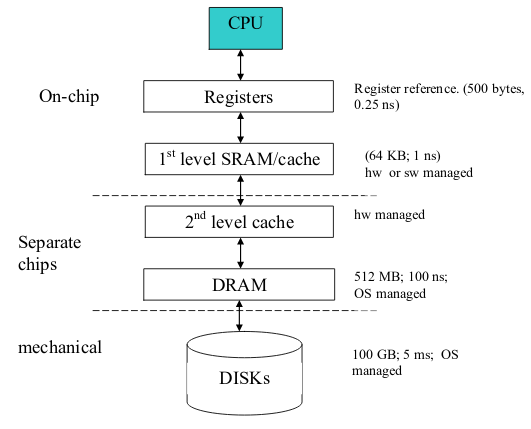
\includegraphics[width=.7\textwidth]{images/memory_hierarchy.png}
Hierarchies work well because memory access follows the principle of locality.

\paragraph{Locality}
\begin{itemize}
    \item \textbf{Temporal locality}:\\
    when a memory entry is referenced, with high probability it will be referenced again within a short time.
    
    \item \textbf{Spatial locality}:\\
    whenever a memory entry is referenced, with high probability reference will be made shortly to neighboring items.
\end{itemize}

\paragraph{Registers}
Registers are usually “exposed” to the programmer. Alternatively, the compiler allocates variables to registers.
Registers are usually placed into a regular register file. A register file consists of multiple read/write ports to allow parallel, simultaneous data accesses.
Typically, at least 2 read and 1 write ports are required to access operands of a single instruction.

Unfortunately, the size of the register file grows with the square of the number of ports so an excessive number of ports slows down the processors.

This quadratic increase in chip area is mostly due to the new additional input and output lines:\\
• Routing problems\\
• Internal bit cell loading increases -> larger power consumption\\
• Linear increment in delay with the number of ports

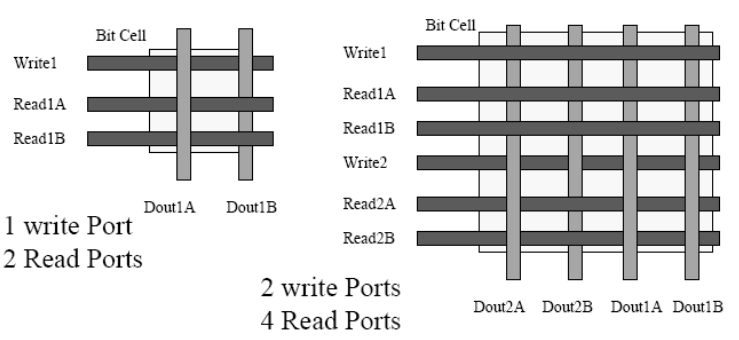
\includegraphics[width=.7\textwidth]{images/memory_bit_cells.png}

It is not profitable to have a register file with more than 15-20 ports: 12 is actually the best tradeoff when number of FU is larger than 4

\paragraph{The usual SRAM}
\begin{itemize}
    \item It is “exposed” to programmer and compiler
    \item Data transfers from/to memory are performed by \textbf{software}
    \item It is mostly used in low-end or specialized embedded processors where worst-case latency to recover data and power are the main issues
\end{itemize}

\paragraph{Cache}
\begin{itemize}
    \item Usually it is “transparent” to programmer and compiler
    \item Transfers from/to lower-level memories are performed by \textbf{hardware}
    \item It is mostly used in high-end processors where the power is less critical and average performance should be maximized
\end{itemize}

\paragraph{Scratch Pad}
It's a low power consumption solution.
The scratch pad is a buffer of memory (no cache) where most frequently used program functions instructions and data are allocated.
This approach requires a preliminary “profiling”to decide what instructions have to be placed into the scratch pad.
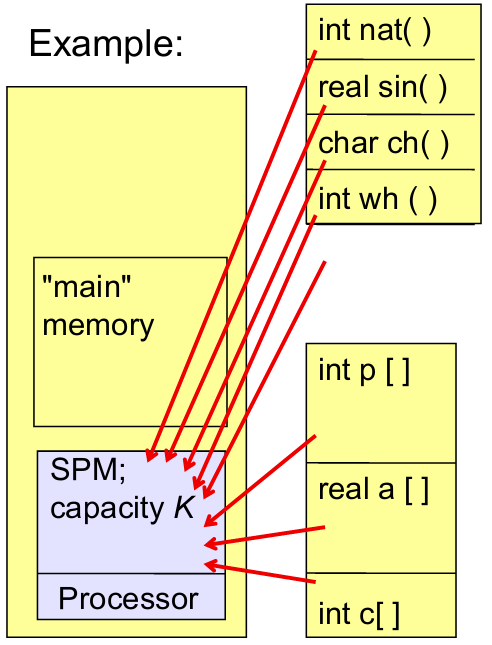
\includegraphics[width=.5\textwidth]{images/memory_scratch_pad.png}
Allocation usually performed statically at compile time (no HW support).
This kind of solution is very used in embedded systems because the program is usually fixed and it is a reasonable tradeoff between performance and power consumption.

\paragraph{Cache}
A cache is a special kind of memory based on SRAM cells which is used to store the data having the maximum probability to be used.
Cache can be either unified (i.e., simultaneously instruction-and data-cache) or split into I-cache and D-cache.

Definitions:
\begin{itemize}
    \item \textbf{Hit}: the item requested by the CPU is present in cache
    \item \textbf{Miss}: the item requested by the CPU is not present in cache
    \item \textbf{Hit rate}: fraction of memory accesses rewarded by hit
    \item \textbf{Miss rate}: fraction of memory accesses resulting in a miss (miss rate = 1 -hit rate)
    \item \textbf{Hit time}: access time (or clock cycles) to cache in the case of success (includes time to determine whether access is met by hit or miss)
    \item \textbf{Miss penalty}: time (or clock cycles) required to substitute a block of data in cache with another block from the lower-level storage
    \item \textbf{Miss time}: miss penalty + hit time, time required to obtain requested data in the case of miss
\end{itemize}

Cache performance is given in terms of average memory access time (AMAT)

$AMAT = hit-time + miss-rate * miss-penalty$\\

Cache performance affects CPU time

$CPU_{time} = IC * (CPI_{execution} + \frac{MEM_{accesses}}{IC} * miss-rate * miss-penalty) * T_{CLK}$

\paragraph{How cache works}
A cache is made of a number of \textbf{blocks} that contain \textbf{words} from memory.
The size of a block is a power of 2, to simplify addressing (e.g., a block is made of 32 words).
When a word is needed, its entire block is loaded from memory and placed somewhere in the cache.
Blocks that are next to each other in memory are not necessarily stored next to each other in the cache, and vice-versa.

The cache needs to store a block along with its actual address in memory.
The required address is compared to the address of all the blocks in the cache to find a match.
If found, it is a hit, otherwise it is a miss.

\paragraph{Problems in cache design}
\begin{itemize}
    \item \textbf{Placement problem}:\\
    Where to place a block transferred from lower to higher level
    \item \textbf{Search (or identification) problem}:\\
    how to determine whether the requested item is present or not
    \item \textbf{Substitution (or replacement) problem}:\\
    Which block present in the cache must be replaced by one in lower-level storage, in the case of a miss
    \item \textbf{Write strategy}:\\
    what happens when a write-to-memory instructions is executed?
\end{itemize}

\section{Direct-mapped cache}


